% THIS TEMPLATE IS A WORK IN PROGRESS

\documentclass{article}

\usepackage{hyperref}
\usepackage{fancyhdr}
\usepackage{graphicx}
\usepackage{cite}
\usepackage[parfill]{parskip}

%\lhead{\includegraphics[width=0.2\textwidth]{nyush-logo.pdf}}
\fancypagestyle{firstpage}{%
  \lhead{NYU Shanghai}
  \rhead{
  %%%% COMMENT OUT / UNCOMMENT THE LINES BELOW TO FIT WITH YOUR MAJOR(S)
  %\&
  %Data
   Machine Learning 2021}
}

%%%% PROJECT TITLE
\title{The Classification of Garbage Based on Chinese Garbage Polity}

%%%% NAMES OF ALL THE STUDENTS INVOLVED (first-name last-name)
\author{\href{mailto:cw3923@nyu.edu}{Chenyang Wen}, \href{mailto:ct2831@nyu.edu}{Chenyu Tang},
\href{mailto:jg5315@nyu.edu}{Jiacheng Guo}}

\date{\vspace{-5ex}} %NO DATE


\begin{document}
\maketitle
\thispagestyle{firstpage}


\begin{abstract}
    In this project, we want to develop a model that can classify garbage photos according to Shanghai garbage classification standards. For those new to Shanghai, such as us new NYU students, facing various of garbage, it is more troublesome to frequently check the standard. We choose three neural networks to build our model, CNN, WasteCNN and Res18. And Res18 has the best performance. And the accuracy of Res18 model reach to 90\%.
\end{abstract}


\section*{Introduction}
In Shanghai, garbage classification has been implemented for more than 20 years. Meanwhile, the classification standard has changed many times. Published on July 1, 2019, Shanghai Municipal Household Garbage Management Regulations divides the classification standard into four categories: recyclable waste, residual waste, household waste and hazardous waste. The strict implementation with high quality of garbage classification cannot be separated from the accurate classification by every citizen in Shanghai. In this project, we want to develop a framework to automatic garbage categorization.

\begin{figure}[!h]
    \begin{centering}
    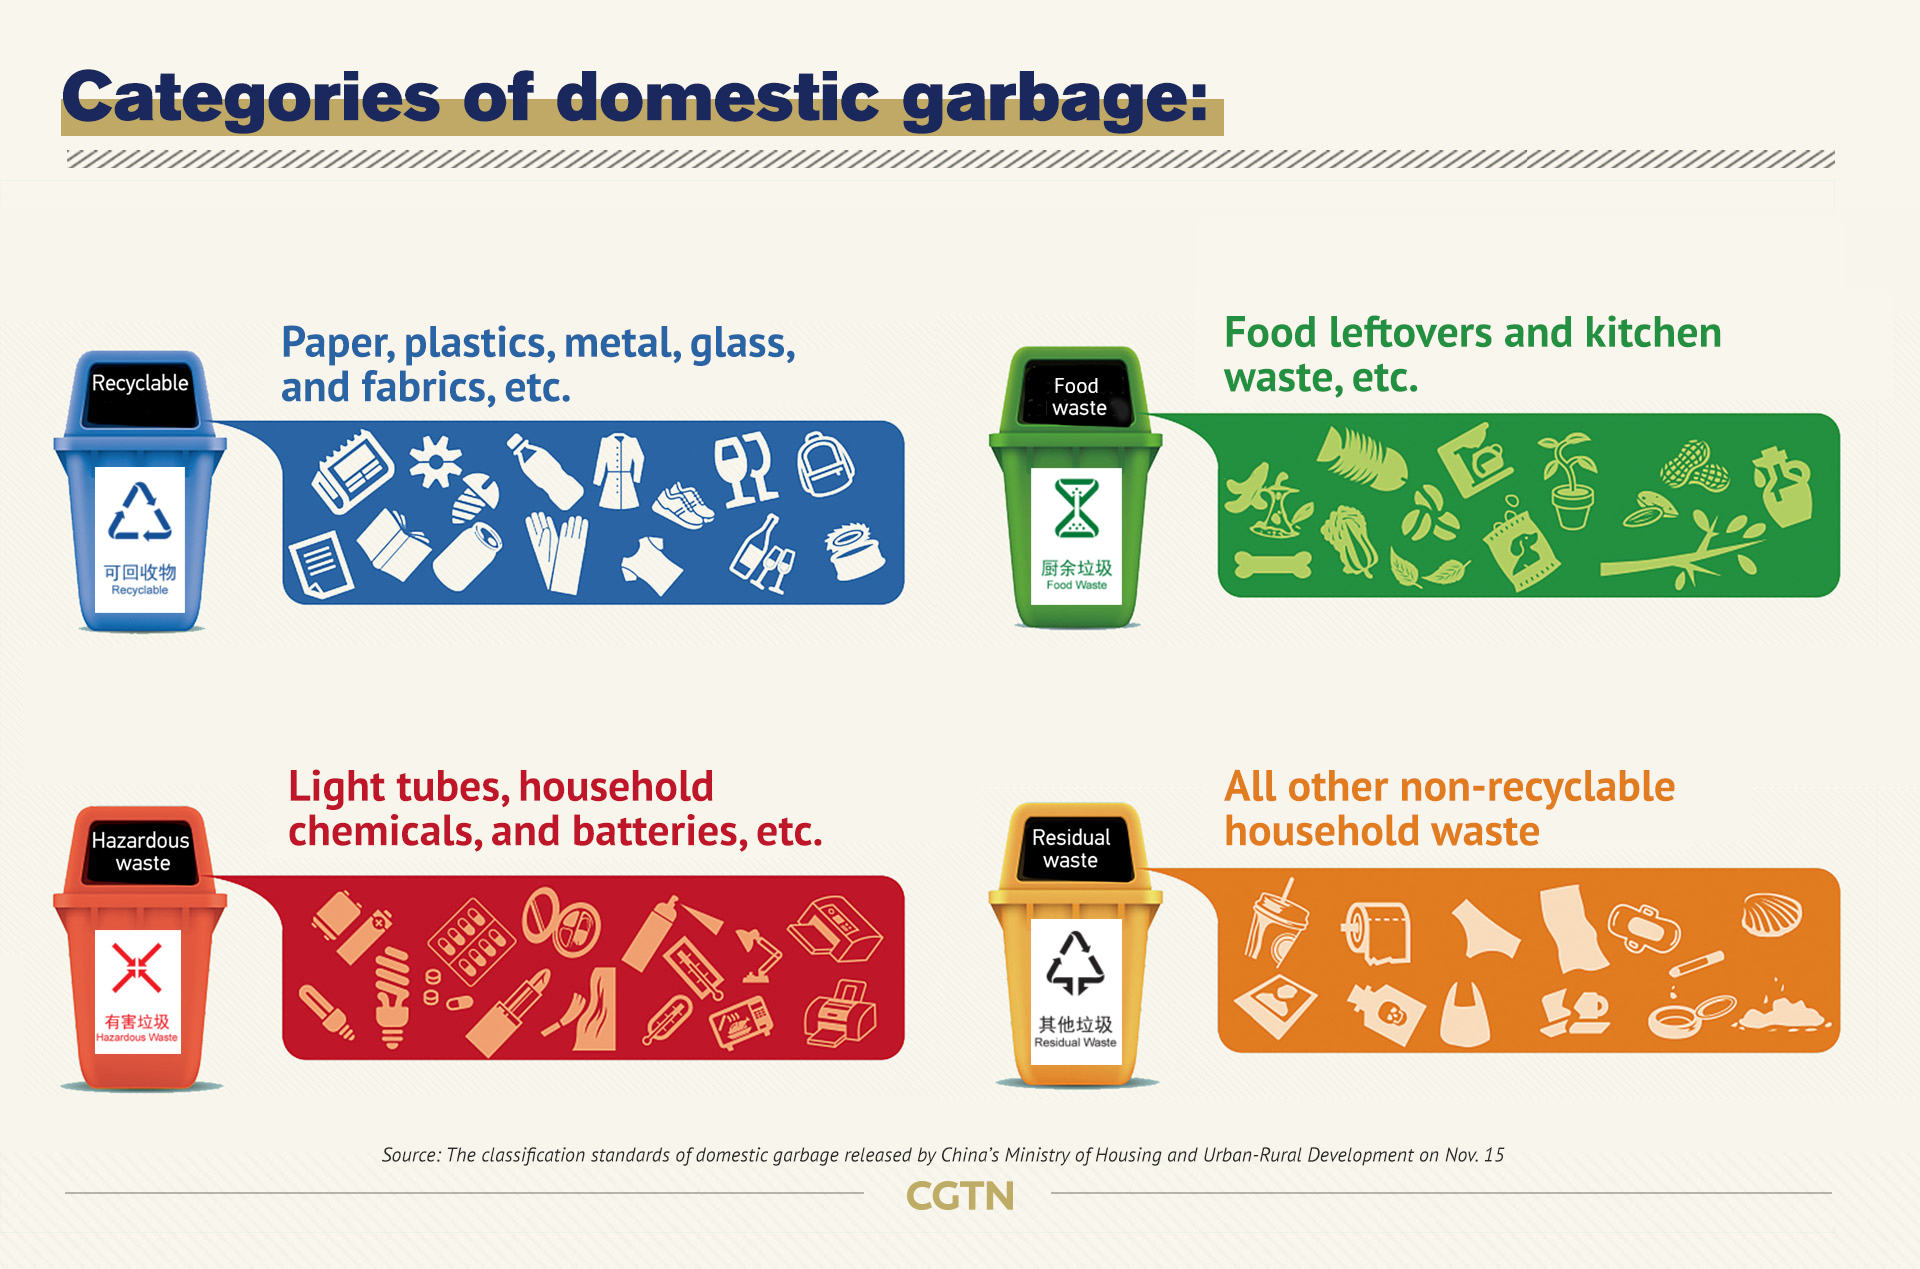
\includegraphics[width=0.95\textwidth]{categories.jpeg}
    \par\end{centering}
    \caption{Standard for waste classification from CGTN\cite{cgtn}}
    \label{fig:Trash_classification}
\end{figure}

Similar to how people identify garbage categories, we want our framework to be able to output garbage categories when it sees the garbage (i.e., the input image). The first step in this process requires the ability to recognize the content of the input image. In the field of image identification, machine learning, especially convolutional neural networks\cite{lecun1995convolutional}, has huge advantages. After get the preprocessed image, our method needs to classify it.



\section*{Dataset}

In this project, dataset is images about garbage. We found two original datasets from garbage classification topic in the Kaggle platform\cite{Kaggle_dataset_6,Kaggle_dataset_12}. The two datasets contain thousands of pictures of more than a dozen different types of garbage. We reassign four labels to the source dataset: recyclable trash, dry trash, wet trash and poison trash. For example, scrap metal and waste plastic relabeled as recyclable trash. In this way, the dataset that meets the requirements of the project is obtained, which contains thousands of images and four labeled garbage types.


\section*{Solution}

    \subsection*{Data Pre-processing}
    For the ideal training efficiency and preventing over-fitting of the model, the following steps are used to preprocess the original data.
    
        \subsubsection*{Image Resize}
        Original images have different resolution. We resize them into 128 * 128 pixel. It ensures a relatively fast training efficiency.
        
        \subsubsection*{Image Normalize}
        In our model, input images are treated as matrix of the value for 3 color channels, R, G and B. Therefore, we need to normalize these values to a normal distribution N(0, 1).
        
        \subsubsection*{Random Transform}
        In this project, various of image transformations are prepared. Each image will randomly select one of the transformations to prevent the model from overfitting and enhance the anti-interference ability of the model. The following transformations are prepared.
        
        \begin{table}[!h]
            \centering
            \begin{tabular}{ |p{1.5cm}|p{1.5cm}|p{1.5cm}|p{1.5cm}|p{1.5cm}|p{1.5cm}|p{1.5cm}|  }
                \hline
                    Original & Flip horizontal & Flip vertical & Rotation randomly & Gaussian blur & Gray \\
                \hline
                    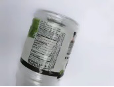
\includegraphics[scale=0.85]{ori.png} & 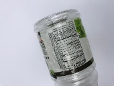
\includegraphics[scale=0.85]{flip_hrz.png} & 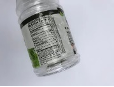
\includegraphics[scale=0.85]{flip_vert.png} &
                    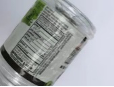
\includegraphics[scale=0.85]{rotation_rand.png} &
                    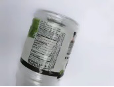
\includegraphics[scale=0.85]{gaussian_blur.png} &
                    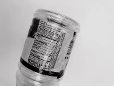
\includegraphics[scale=0.85]{gray.png}\\
                \hline
            \end{tabular}
            \caption{Value of precision, recall and F1-score}
            \label{tab:pre_rec_f1}
        \end{table}
        
        \subsubsection*{Data Split}
        After random transform, well-processed data is divided into training set, validation set and test set. The proportions of the three are respectively 72\%, 18\% and 10\%. Then these three sets are read into the model in the format of Dataloader class, for the following model training and evaluation.
    

    \subsection*{Neural Network \& Model Selection}
    Neural network has already taken a place for many years. Based on the practical experience and experiment result, it performed pretty well, even better than the traditional machine learning algorithm. And the convolutional neural network is one of the main categories to do computer vision tasks both in recognition and classification. Since the project is based on the image classification, the most common way to classify the image for now is to use deep neural network. And this is also the most mature way in computer vision, so we here specify three different network for training.
    The basic CNN with 2 convolution layers and 3 fully connected layers that for garbage classification tasks is as the base line for the improvement of other models. And compare with the basic CNN, wasteCNN add one convolutional layer addition for improvement; and another neural network is Res18, inspired by the original ResNet\cite{he2016deep}, cascading with previous layers. This kind of skip connection let the network able to preserve the feature from previous layers, make the network much easier to preserve the gradient.


    \subsection*{Models Construction \& Training}
    And as for the model chosen process, if the model is much deeper, then the time consuming for training process will be much longer, so the res18 is the deepest network we choose. It is true that the Res50 will have much deeper network and similar amount of parameter with the network that applied with ResNet. So it is also the network we want to realize by ourselves, but these are sufficient models to classify the garbage by these models and choose the best one. As for network parameter, all the convolutional kernels including the first layer of Res18 are using $3\times3$ large to reduce the parameter number, stride set default as 1 except some layers within Res18 for downsampling.
    
        \subsubsection*{CNN}
        This is the most basic model applied in the project. The model's input, which is the image size is 128. And adjust the image size will also affect the model’s first fully connected layer's neuron's number. Since the structure is similar as wasteCNN, so we won't specific shown the structure figure here.

        \subsubsection*{WasteCNN}
        The model structure is shown in Figure \ref{fig:wasteNet_model} with the image size is 128, adjusting the image size will affect the model’s first fully connected layer. Basic backbone is as same as CNN. The difference is that there is 3 convolutional layers and larger fully connected layer.
        \begin{figure}[!h]
            \begin{centering}
            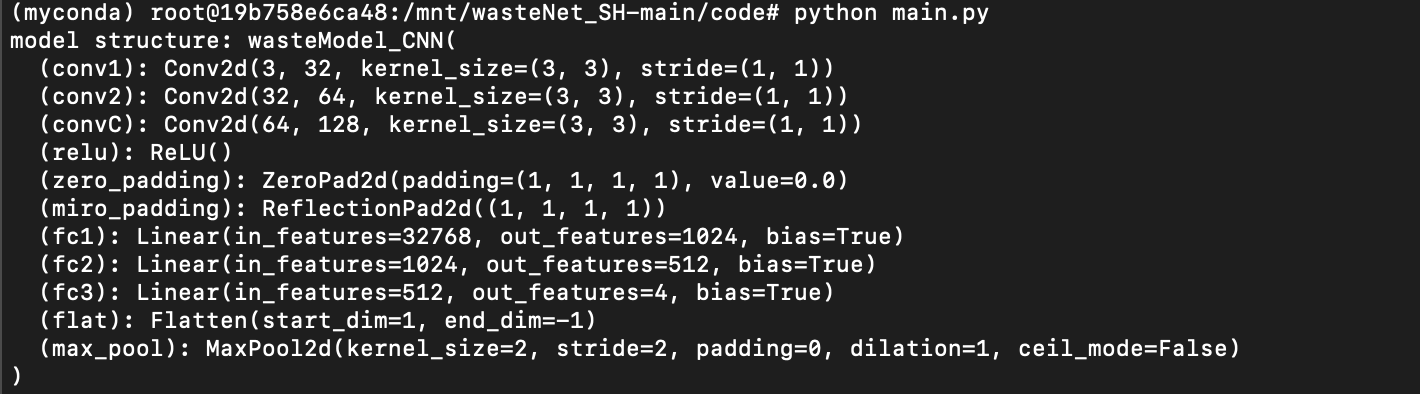
\includegraphics[width=0.95\textwidth]{wasteCNN.png}
            \par\end{centering}
            \caption{wasteCNN model structure}
            \label{fig:wasteNet_model}
        \end{figure}

        \subsubsection*{Res18}
        Res18 has 18 convolutional layers. First thing is to construct the ResBlock, which is the basic component for the ResNet. ResBlock is built by two convolutional layers and a shortcut, which represent the combination of current Conv layer output and previous output. Then connect with 4 blocks and addition 1 Conv layer in the front and 1 fully connected layer at the end. And the part of ResNet is also shown as Figure \ref{fig:res18_model}.
        \begin{figure}[!h]
            \begin{centering}
            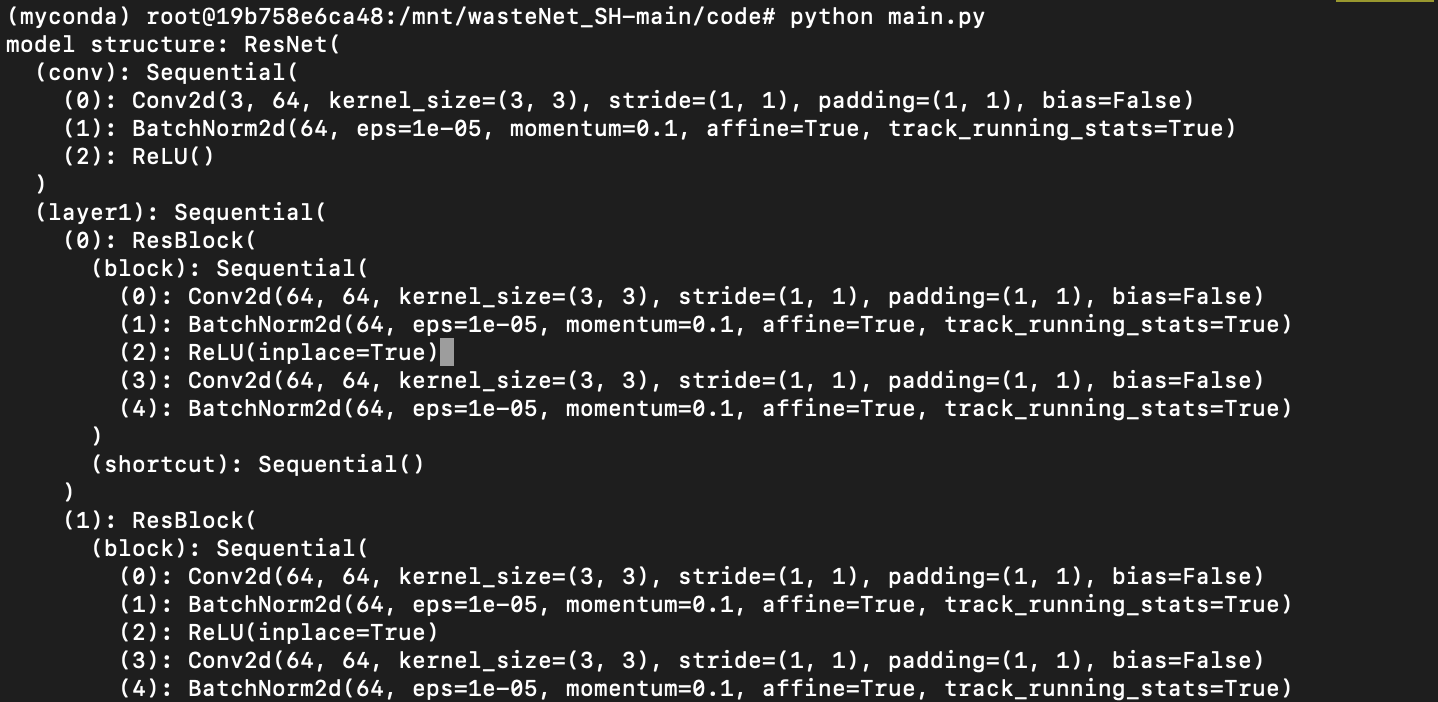
\includegraphics[width=0.95\textwidth]{Res18.png}
            \par\end{centering}
            \caption{Part of ResNet with 18 convolutional layer}
            \label{fig:res18_model}
        \end{figure}
        
        \subsubsection*{Loss Function}
        Since the project is classification problem, so the cross-entropy loss is chosen as the loss function. And here is the loss function.
        \begin{equation}
            J(w)=-\Sigma^N_{i=1}\{y_ilogp(x_i;w)+(1-y_i)log(1-p(x_i;w))\}
        \end{equation}
        
        Other sets of training are: `batch size': 32, `validation data's percentage': 0.2, `learning rate': 1e-3, `epoch': 50, and if the code is running on GPU is much quicker.

\section*{Results and Discussion}
The project separately evaluates these three kinds of models by using many evaluation methods and obtained the following figures and results: the variation curve of Test Accuracy with the number of epochs shown as Figure \ref{fig:Accuracy}. And the variation curve of AUC value with the number of epochs as Figure \ref{fig:AUC}.

\begin{figure}[!h]
    \begin{centering}
    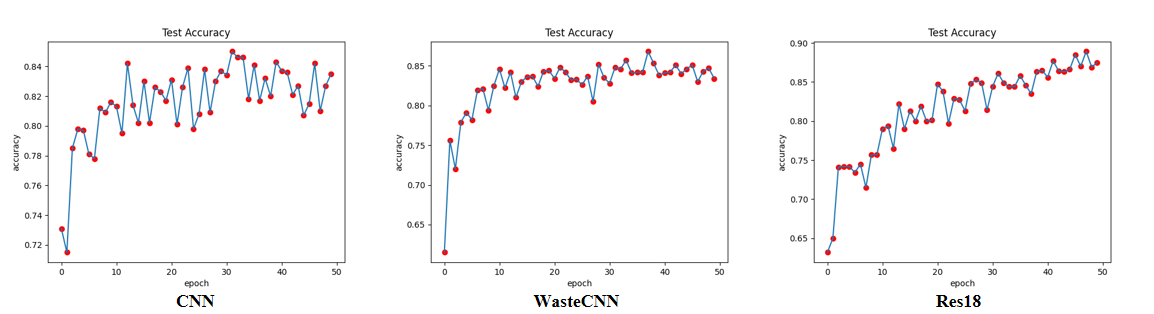
\includegraphics[width=0.95\textwidth]{accuracy.png}
    \par\end{centering}
    \caption{Accuracy-Epoch Curve}
    \label{fig:Accuracy}
\end{figure}

\begin{figure}[!h]
    \begin{centering}
    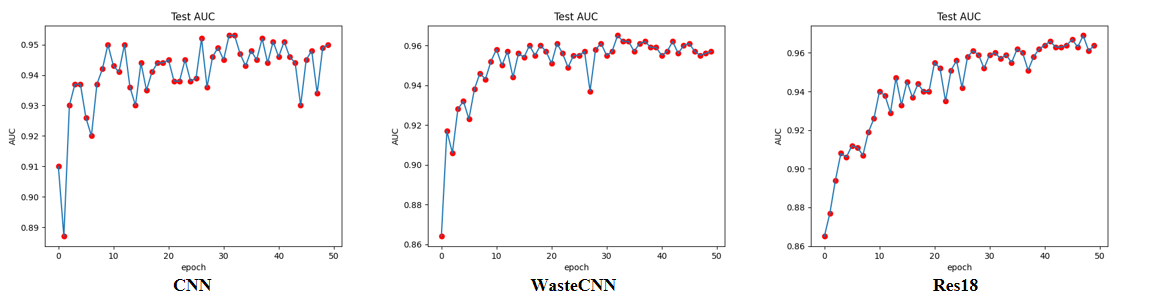
\includegraphics[width=0.95\textwidth]{AUC.png}
    \par\end{centering}
    \caption{AUC value-Epoch Curve}
    \label{fig:AUC}
\end{figure}

According to figures \ref{fig:Accuracy} and \ref{fig:AUC}, the project selects the iteration that performs better in the test dataset and get the confusion matrix and ROC curve (after averaging the four categories) under that iteration. Then calculate the Precision, Recall for each category.

\begin{figure}[!h]
    \begin{centering}
    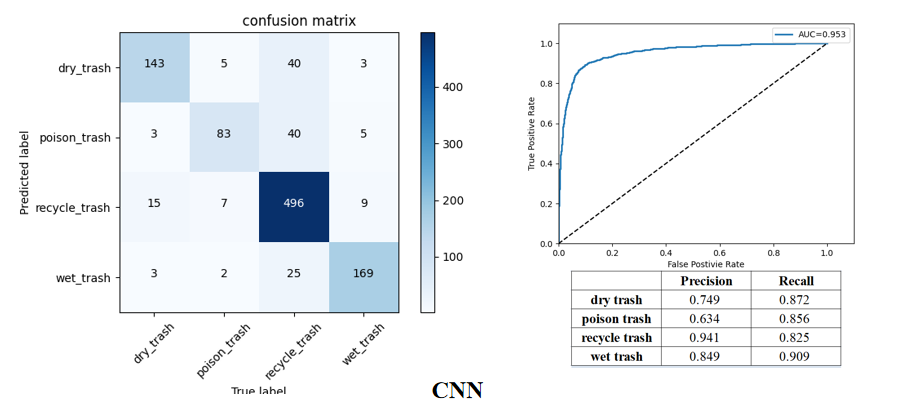
\includegraphics[width=0.95\textwidth]{CNN_eva.png}
    \par\end{centering}
    \caption{Confusion metrics and ROC curves of CNN}
    \label{fig:CNN_confusion_ROC}
\end{figure}

\begin{figure}[!h]
    \begin{centering}
    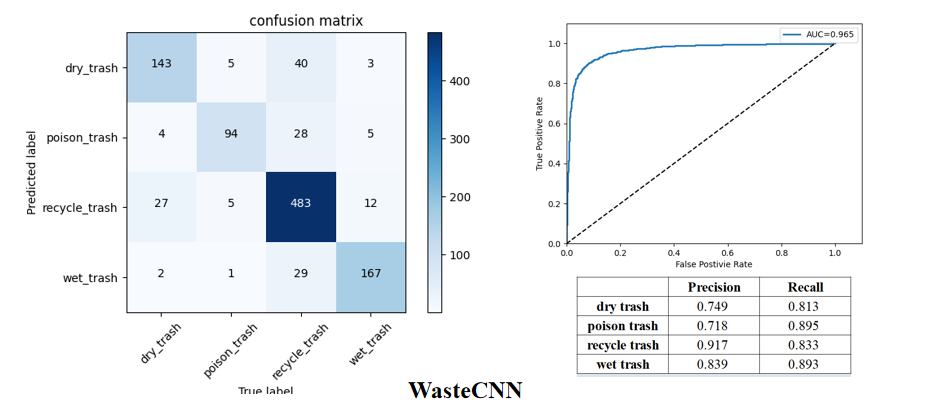
\includegraphics[width=0.95\textwidth]{WasteCNN_eva.png}
    \par\end{centering}
    \caption{Confusion metrics and ROC curves of WasteCNN}
    \label{fig:WasteCNN_confusion_ROC}
\end{figure}

\begin{figure}[!h]
    \begin{centering}
    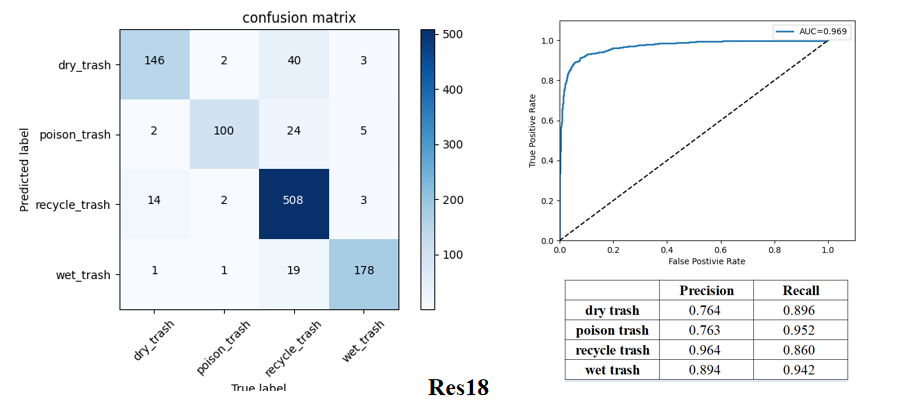
\includegraphics[width=0.95\textwidth]{Res18_eva.png}
    \par\end{centering}
    \caption{Confusion metrics and ROC curves of Res18}
    \label{fig:Res18_confusion_ROC}
\end{figure}


Due to the uneven distribution of data in the test set, the project decides to calculate the macro average and micro average of precision, recall and F1-score of the three models respectively to compare the performance. The work result is shown at Table \ref{tab:pre_rec_f1}.

\begin{table}[!h]
    \centering
    \begin{tabular}{ |p{2cm}||p{2cm}|p{2cm}|p{2cm}|  }
        \hline
            \multicolumn{4}{|c|}{Macro average} \\
        \hline
             & Precision &Recall&F1-score\\
        \hline
            CNN    &   0.793   &   0.865  &    0.828\\
            WasteCNN    &   0.805   &   0.858   &   0.831\\
            Res18   &   0.847   &   0.912   &   0.878\\
        \hline\hline
            \multicolumn{4}{|c|}{Micro average} \\
        \hline
             & Precision &Recall&F1-score\\
        \hline
            CNN    &   0.850   &   0.850  &    0.850\\
            WasteCNN    &   0.846   &   0.846   &   0.846\\
            Res18   &   0.889   &   0.889   &   0.889\\
        \hline
    \end{tabular}
    \caption{Value of precision, recall and F1-score}
    \label{tab:pre_rec_f1}
\end{table}

These results shows that Res18 model has the highest accuracy when predicting the test dataset, accuracy is up to 89\% within 50 iterations, while the accuracy of CNN and wasteCNN models is about 83\% and 85\%. In addition, the average Precision, Recall and F1-score values of the Res18 model are also the closest to ``1". The Precision, Recall and F1-score calculated by macro and micro average methods are basically the same, indicating the accuracy of classification is not affected by the number of samples in different categories. The AUC value of Res18 model is up to 0.97 within 50 iterations, which is also higher than in the wasteCNN and CNN models. Hence, it can be seen that Res18 model is the most accurate in the classification of garbage pictures among these three models.
In the case of calculating the values of precision and recall by category of garbage, there is little difference in the value of recall for different categories in three models, but the value of precision for recyclable trash, which is up to 0.96 in Res18 model, is 0.2 more than that for dry trash and poison trash categories. This problem needs further study.

\nocite{*}
\bibliographystyle{IEEEtran}
\bibliography{references}

\end{document}
